\begin{figure}[h]
    \centering
    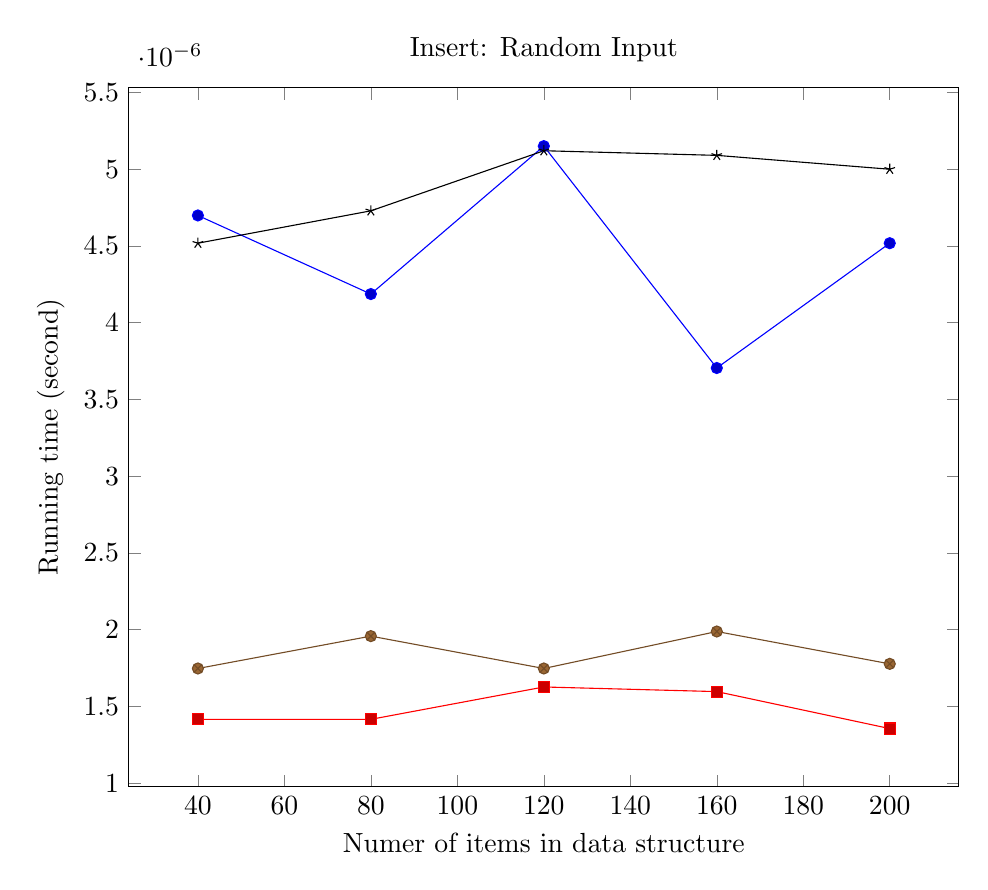
\begin{tikzpicture}
        \begin{axis}[
            xlabel={Numer of items in data structure},
            ylabel={Running time (second)},
            title={Insert: Random Input},
            width=\textwidth
        ]
		\addplot coordinates {
			(40, 4.698335253325997e-06)
			(80, 4.186337180848293e-06)
			(120, 5.15009825845375e-06)
			(160, 3.7044566420452175e-06)
			(200, 4.5176300512754505e-06)
		};
		\addplot coordinates {
			(40, 1.4155240827325166e-06)
			(80, 1.4155240827332105e-06)
			(120, 1.626346818459079e-06)
			(160, 1.5962292847837566e-06)
			(200, 1.355289015381872e-06)
		};
		\addplot coordinates {
			(40, 1.7468169531596745e-06)
			(80, 1.9576396888862367e-06)
			(120, 1.7468169531596745e-06)
			(160, 1.9877572225608653e-06)
			(200, 1.7769344868349969e-06)
		};
		\addplot coordinates {
			(40, 4.5176300512754505e-06)
			(80, 4.728452787001319e-06)
			(120, 5.119980724778428e-06)
			(160, 5.0898631911038e-06)
			(200, 4.999510590077833e-06)
		};
        \legend{}
        \end{axis}
    \end{tikzpicture}
    \caption{Average of 0 operations, benchmarked every 0, starting at 0.}
\end{figure}